\section{Quantitative Analysis}

\subsection{Combining the facets Contribution, SLA Usage and Data Integration Description}

\begin{figure}[h!]
\centering
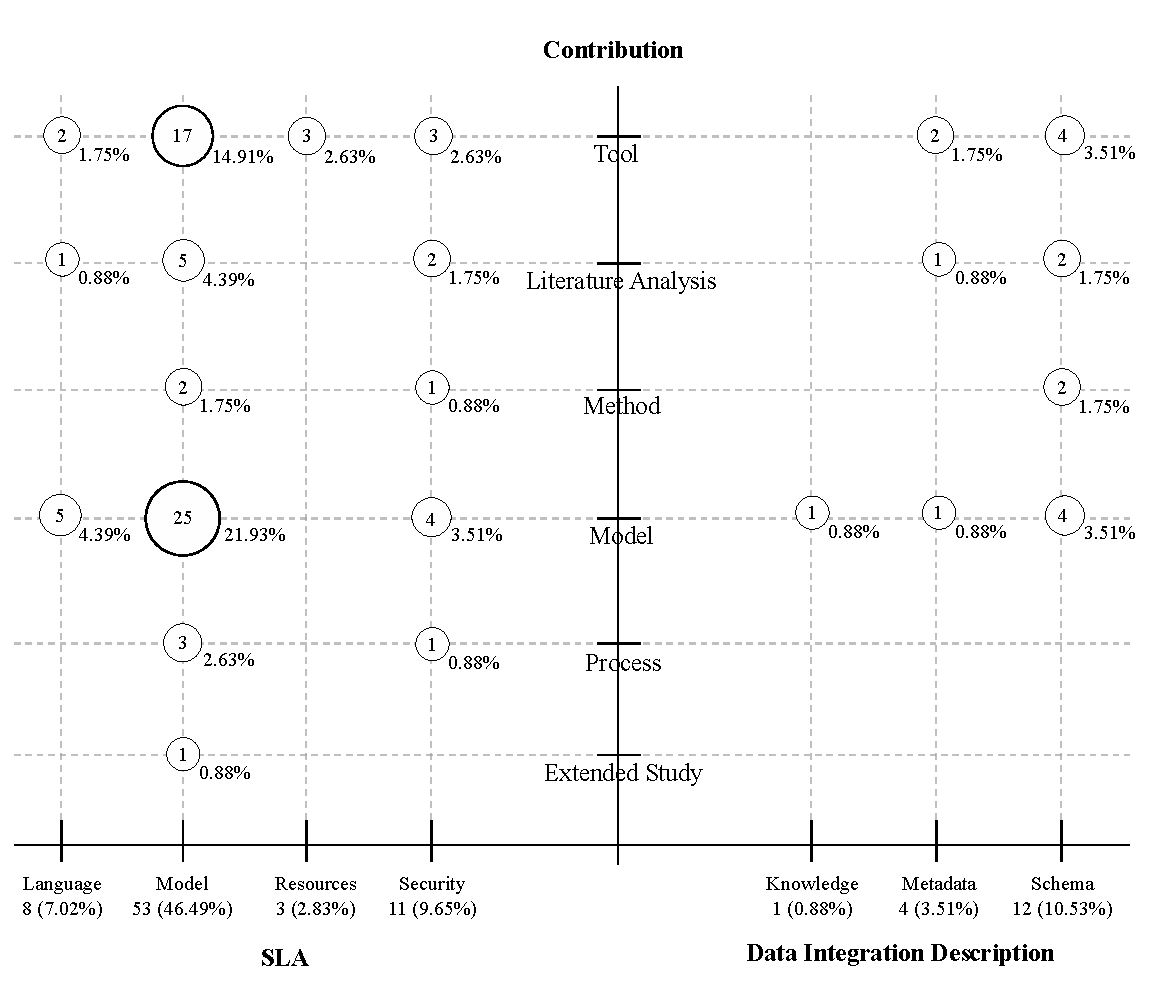
\includegraphics[scale=0.5]{figs/bubble-charts/Contribution-SLA-DIdescription.pdf} 
\caption{Contribution, SLA Usage and Data Integration Description}\label{fig:facet1}
\end{figure}

\subsection{Combining the facets Data Integration Environment, Contribution and Research}

\begin{figure}[h!]
\centering
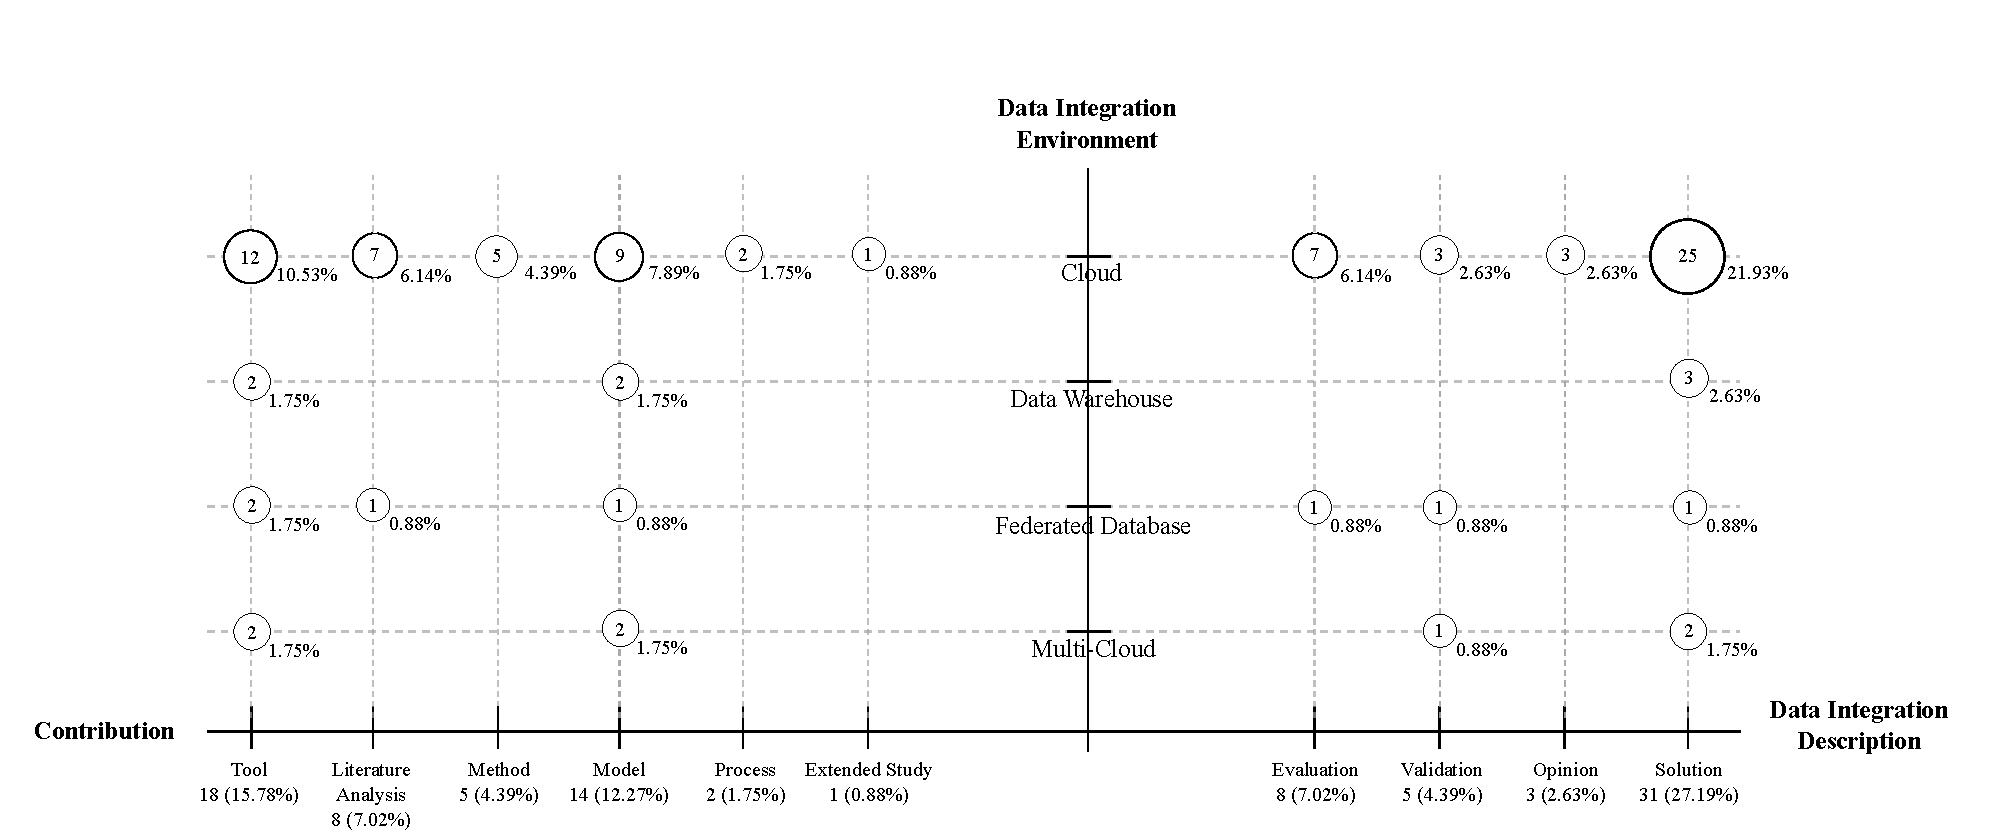
\includegraphics[scale=0.5]{figs/bubble-charts/DI-Environment-Contribution-Research.pdf}
\caption{facets Data Integration Environment, Contribution and Research}\label{fig:facet2}
\end{figure}

\subsection{Combining the facets SLA Usage and Contribution}

\begin{figure}[h!]
\centering
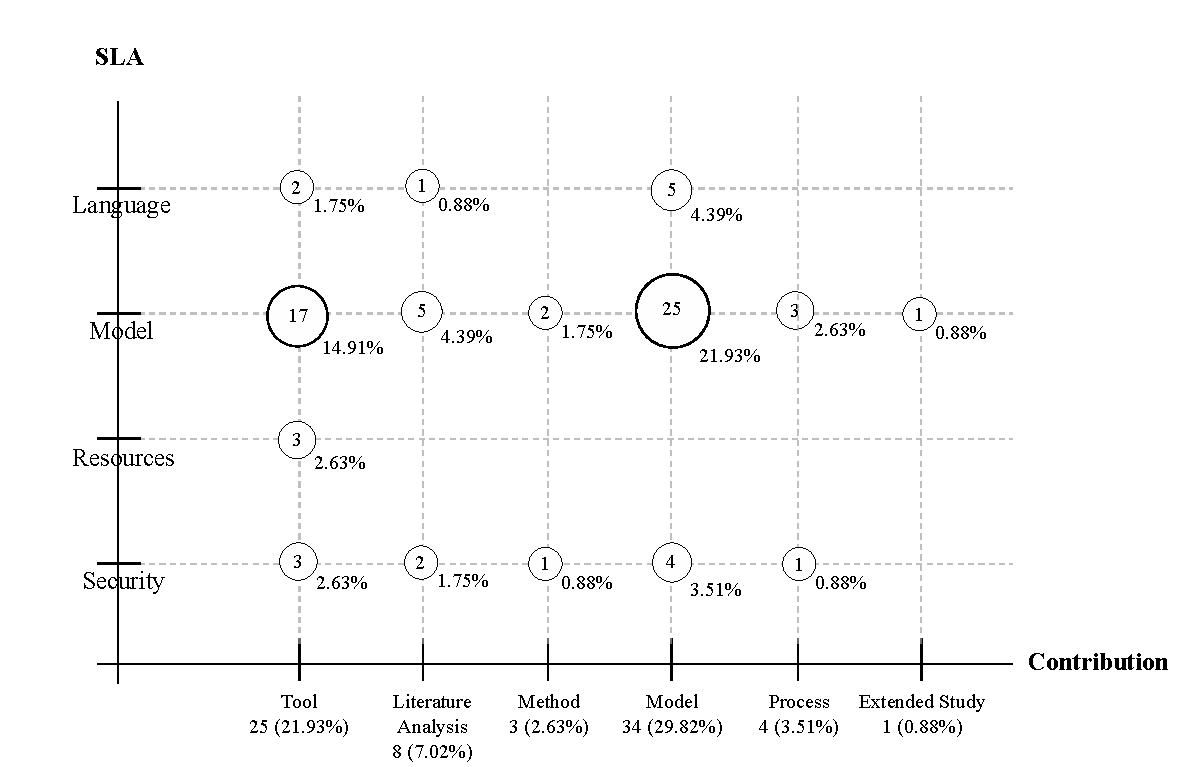
\includegraphics[scale=0.5]{figs/bubble-charts/SLA-Contribution.pdf}
\caption{Facets SLA Usage and Contribution}\label{fig:facet3}
\end{figure}


\subsection{Combining the facets Data Quality, Data Integration Environment and Data Integration Description}

Combining the facet Data Quality with the facets Data Integration Environment e Data Integration Description
(Figure~\ref{fig:facet4}) it is possible to note which quality of service parameters have been applied most in
data integration studies.
It is also possible to identify which are the most applied data integration environment and description.
First of all, security and privacy are the most applied QoS parameter (5 appearance - 4.39\%)
followed by the other dimensions (1 appearance - 0.88\%). 
The figure also shows that SLA has not been widely used in order to address data integration solutions
(1 appearance) which reinforces our main objective of integrate SLA, data integration and multi-cloud 
environments. 
Analyzing the figure is also possible to observe that the most deployed data integration environment is 
the cloud (9.68\%) followed by multi-cloud (4.39\%), federated databases (1.75\%) and data warehouse (0.00\%).
The data integration description dimensions had the same percentage for schema, knowledge and metadata (2 appearance - 1.75\%)

\begin{figure}[h!]
\centering
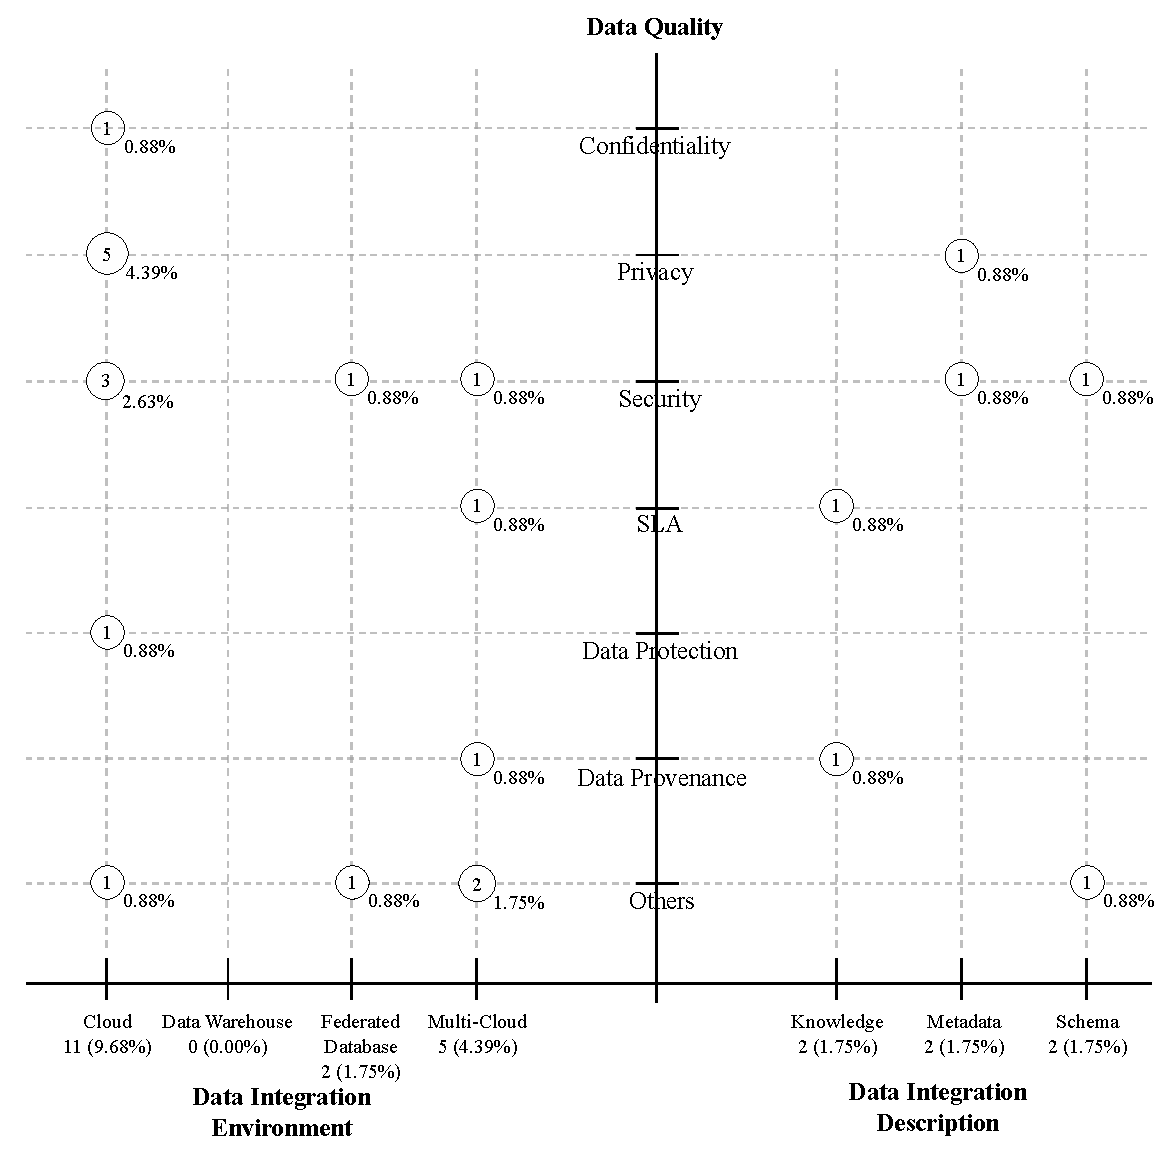
\includegraphics[scale=0.53]{figs/bubble-charts/Data-Quality-DI.pdf}
\caption{Facets Data Quality, Data Integration Environment and Data Integration Description}\label{fig:facet4}
\end{figure}
